\chapter{Additional Source Judgements}

\begin{figure}
\fbox{$\Gamma \vdash_{ty} \sigma$}
\begin{mathpar}
\inferrule*[right=WfVar]
{
  a \in \Gamma
}
{
  \Gamma \vdash_{ty} a
}
\quad
\inferrule*[right=WfCon]
{
}
{
  \Gamma \vdash_{ty} T
}
\quad
\inferrule*[right=WfQual]
{
  \Gamma \vdash_{ty} \sigma
  \\
  \Gamma \vdash_{ct} \pi
}
{
  \Gamma \vdash_{ty} \pi \Rightarrow \sigma
}
\\
\inferrule*[right=WfFam]
{
  \Gamma \vdash_{ty} \tau_i
}
{
  \Gamma \vdash_{ty} F(\overline{\tau})
}
\quad
\inferrule*[right=WfApp]
{
  \Gamma \vdash_{ty} \tau_1
  \\
  \Gamma \vdash_{ty} \tau_2
}
{
  \Gamma \vdash_{ty} \tau_1 \; \tau_2
}
\quad
\inferrule*[right=WfAll]
{
  \Gamma, a \vdash_{ty} \sigma
  \\
  a \notin fv(\Gamma)
}
{
  \Gamma \vdash_{ty} \forall a. \; \sigma
}
\end{mathpar}
\caption{Type Well-formedness}
\end{figure}
\begin{figure}
\begin{mathpar}
\inferrule*[right=WfEq]
{
  \Gamma \vdash_{ty} \tau_1
  \\
  \Gamma \vdash_{ty} \tau_2
}
{
  \Gamma \vdash_{ct} \tau_1 \sim \tau_2
}
\quad
\inferrule*[right=WfCls]
{
  \Gamma \vdash_{ty} \tau_i
}
{
  \Gamma \vdash_{ct} TC \; \overline{\tau}
}
\end{mathpar}
\caption{Constraint Well-formedness}
\end{figure}

\begin{figure}
\fbox{$\Gamma \vdash_{ty} \sigma \rightsquigarrow v$}
\begin{mathpar}
\inferrule*[right=ETyVar]
{
  a \in \Gamma
}
{
  \Gamma \vdash_{ty} a \rightsquigarrow a
}
\quad
\inferrule*[right=ETyCon]
{
}
{
  \Gamma \vdash_{ty} T \rightsquigarrow T
}
\\
\inferrule*[right=ETyQual]
{
  \Gamma \vdash_{ty} \sigma \rightsquigarrow v
  \\
  \Gamma \vdash_{cc} \pi_i \rightsquigarrow v_i
}
{
  \Gamma \vdash_{ty} \overline{\pi} \Rightarrow \sigma \rightsquigarrow \overline{v}
  \rightarrow v
}
\\
\inferrule*[right=ETyFam]
{
  \Gamma \vdash_{ty} \tau_i \rightsquigarrow v_i
}
{
  \Gamma \vdash_{ty} F(\overline{\tau}) \rightsquigarrow F(\overline{v})
}
\quad
\inferrule*[right=ETyApp]
{
  \Gamma \vdash_{ty} \tau_1 \rightsquigarrow v_1
  \\
  \Gamma \vdash_{ty} \tau_2 \rightsquigarrow v_2
}
{
  \Gamma \vdash_{ty} \tau_1 \; \tau_2 \rightsquigarrow v_1 \; v_2
}
\\
\inferrule*[right=ETyAll]
{
  \Gamma, a \vdash_{ty} \sigma \rightsquigarrow v
  \\
  a \notin fv(\Gamma)
}
{
  \Gamma \vdash_{ty} \forall a. \; \sigma \rightsquigarrow \forall a. \; v
}
\end{mathpar}
\caption{Type Translation}
\end{figure}

\begin{figure}
\fbox{$\Gamma \vdash_{eq} \phi \rightsquigarrow \psi$}
\begin{mathpar}
\inferrule*[right=EEqCt]
{
  \Gamma \vdash_{ty} \tau_1 \rightsquigarrow v_1
  \\
  \Gamma \vdash_{ty} \tau_2 \rightsquigarrow v_2
}
{
  \Gamma \vdash_{eq} \tau_1 \sim \tau_2 \rightsquigarrow v_1 \sim v_2
}
\end{mathpar}
\caption{Equality Constraint Translation}
\end{figure}

\begin{figure}
\fbox{$\Gamma \vdash_{eq} \pi \rightsquigarrow v$}
\begin{mathpar}
\inferrule*[right=EClsCt]
{
  \Gamma \vdash_{ty} \tau_i \rightsquigarrow v_i
}
{
  \Gamma \vdash_{ct} TC \; \overline{\tau} \rightsquigarrow T_{TC} \;
  \overline{v}
}
\end{mathpar}
\caption{Class Constraint Translation}
\end{figure}

\chapter{Additional $\text{F}_\text{C}$ Judgements}
\begin{figure}
\fbox{$\Gamma \vdash_d decl \; \Gamma'$}
\begin{mathpar}
\inferrule*[right=Data]
{
  \Gamma, (\overline{a : k}) (\overline{b : k'}) \vdash_{pr} \psi_i
  \\
  \Gamma, (\overline{a : k}) (\overline{b : k'}) \vdash_{ty} v_j
}
{
  \Gamma \vdash_{d} (\textbf{data} \; T \; (\overline{a : k}) \; \textbf{where} \; K :
  \forall (\overline{a : k}) (\overline{b : k'}). \; \overline{\psi} \Rightarrow \overline{v}
  \rightarrow T \; \overline{a}) : \bullet
}
\\
\inferrule*[right=Family]
{
  ~
}
{
  \Gamma \vdash_{d} (\textbf{type} \; F(\overline{a : k}) : k) : \bullet
}
\\
\inferrule*[right=Axiom]
{
  \Gamma, (\overline{a : k}) \vdash_{ty} v_i
  \\
  \Gamma, (\overline{a : k}) \vdash_{ty} v
  \\
  g \notin dom(\Gamma)
}
{
  \Gamma \vdash_{d} (\textbf{axiom} \; g \; (\overline{a : k}) : F(\overline{v}) \sim v)
  : \{g \; (\overline{a : k}) : F(\overline{v}) \sim v\}
}
\\
\inferrule*[right=Value]
{
  \Gamma \vdash_{tm} t : v
  \\
  x \notin dom(\Gamma)
}
{
  \Gamma \vdash_{d} (\textbf{let} \; x : v = t) : \{x : v\}
}
\end{mathpar}
\caption{Declaration Typing}
\end{figure}

\begin{figure}
\fbox{$\Gamma_{co} \vdash_{co} \gamma : \psi$}
\begin{mathpar}
\inferrule*[right=TyCoVar]
{
    (c : \psi) \in \Gamma_{co}
}
{
    \Gamma_{co} \vdash c : \psi
}
\quad
\inferrule*[right=TyCoAx]
{
    (g \; (\overline{a : k}) : v_1 \sim v_2) \in \Gamma_{co}
}
{
    \Gamma_{co} \vdash g \; \overline{v} : [\overline{a} \mapsto \overline{v}]v_1
    \sim [\overline{a} \mapsto \overline{v}]v_2
}
\\
%CoRefl
\inferrule*[right=TyCoRefl]
{
    ~
}
{
    \Gamma_{co} \vdash \langle v \rangle : v \sim v
}
\quad
%CoSym
\inferrule*[right=TyCoSym]
{
    \Gamma_{co} \vdash \gamma : v_1 \sim v_2
}
{
    \Gamma_{co} \vdash \text{sym} \; \gamma : v_2 \sim v_1
}
\\
%CoTrans
\inferrule*[right=TyCoTrans]
{
    \Gamma_{co} \vdash \gamma_1 : v_1 \sim v_2
    \\
    \Gamma_{co} \vdash \gamma_2 : v_2 \sim v_3
}
{
    \Gamma_{co} \vdash \gamma_1 \fctrans \gamma_2 : v_1 \sim v_3
}
\\
%CoApp
\inferrule*[right=TyCoApp]
{
    \Gamma_{co} \vdash \gamma_1 : v_1 \sim v_2
    \\
    \Gamma_{co} \vdash \gamma_2 : v_3 \sim v_4
}
{
    \Gamma_{co} \vdash \gamma_1 \; \gamma_2 : v_1 \; v_3 \sim v_2 \; v_4
}
\\
%CoLeft
\inferrule*[right=TyCoLeft]
{
    \Gamma_{co} \vdash \gamma : v_1 \; v_2 \sim v_3 \; v_4
}
{
    \Gamma_{co} \vdash \text{left} \; \gamma : v_1 \sim v_3
}
\quad
%CoRight
\inferrule*[right=TyCoRight]
{
    \Gamma_{co} \vdash \gamma : v_1 \; v_2 \sim v_3 \; v_4
}
{
    \Gamma_{co} \vdash \text{right} \; \gamma : v_2 \sim v_4
}
\\
%CoFam
\inferrule*[right=TyCoFam]
{
    \overline{\Gamma_{co} \vdash \gamma : v_1 \sim v_2}
}
{
    \Gamma_{co} \vdash_{co} F(\overline{\gamma}) : F(\overline{v_1}) \sim
    F(\overline{v_2})
}
\quad
%CoAbs
\inferrule*[right=TyCoAbs]
{
    \Gamma_{co}, a : k \vdash_{co} \gamma : v_1 \sim v_2
}
{
    \Gamma_{co} \vdash_{co} \forall a. \; \gamma : \forall. a \; v_1 \sim \forall. a
    \; v_2
}
\\
%CoInst
\inferrule*[right=TyCoInst]
{
    \Gamma_{co} \vdash \forall a. \; \gamma_1 : \forall. a \; v_1 \sim \forall. a
    \; v_2
    \\
    \Gamma_{co} \vdash \gamma_2 : v_3 \sim v_4
}
{
    \Gamma_{co} \vdash \gamma_1 [\gamma_2] : [a \mapsto v_3]v_1 \sim [a \mapsto
    v_4]v_2
}
\\
%CoQual
\inferrule*[right=TyCoQual]
{
    \Gamma_{co} \vdash \gamma : v_1 \sim v_2
}
{
    \Gamma_{co} \vdash \psi \Rightarrow \gamma : (\psi \Rightarrow v_1) \sim
    (\psi \Rightarrow v_2)
}
\\
%CoQual
\inferrule*[right=TyCoQInst]
{
    \Gamma_{co} \vdash \gamma_1 : (\psi \Rightarrow v_1) \sim
    (\psi \Rightarrow v_2)
}
{
    \Gamma_{co} \vdash \gamma_1 @ \gamma_2 : v_1 \sim v_2
}
\end{mathpar}
\caption{Simplified Coercion Typing}
\label{fig:fc-co-type}
\end{figure}

\chapter{Poster}
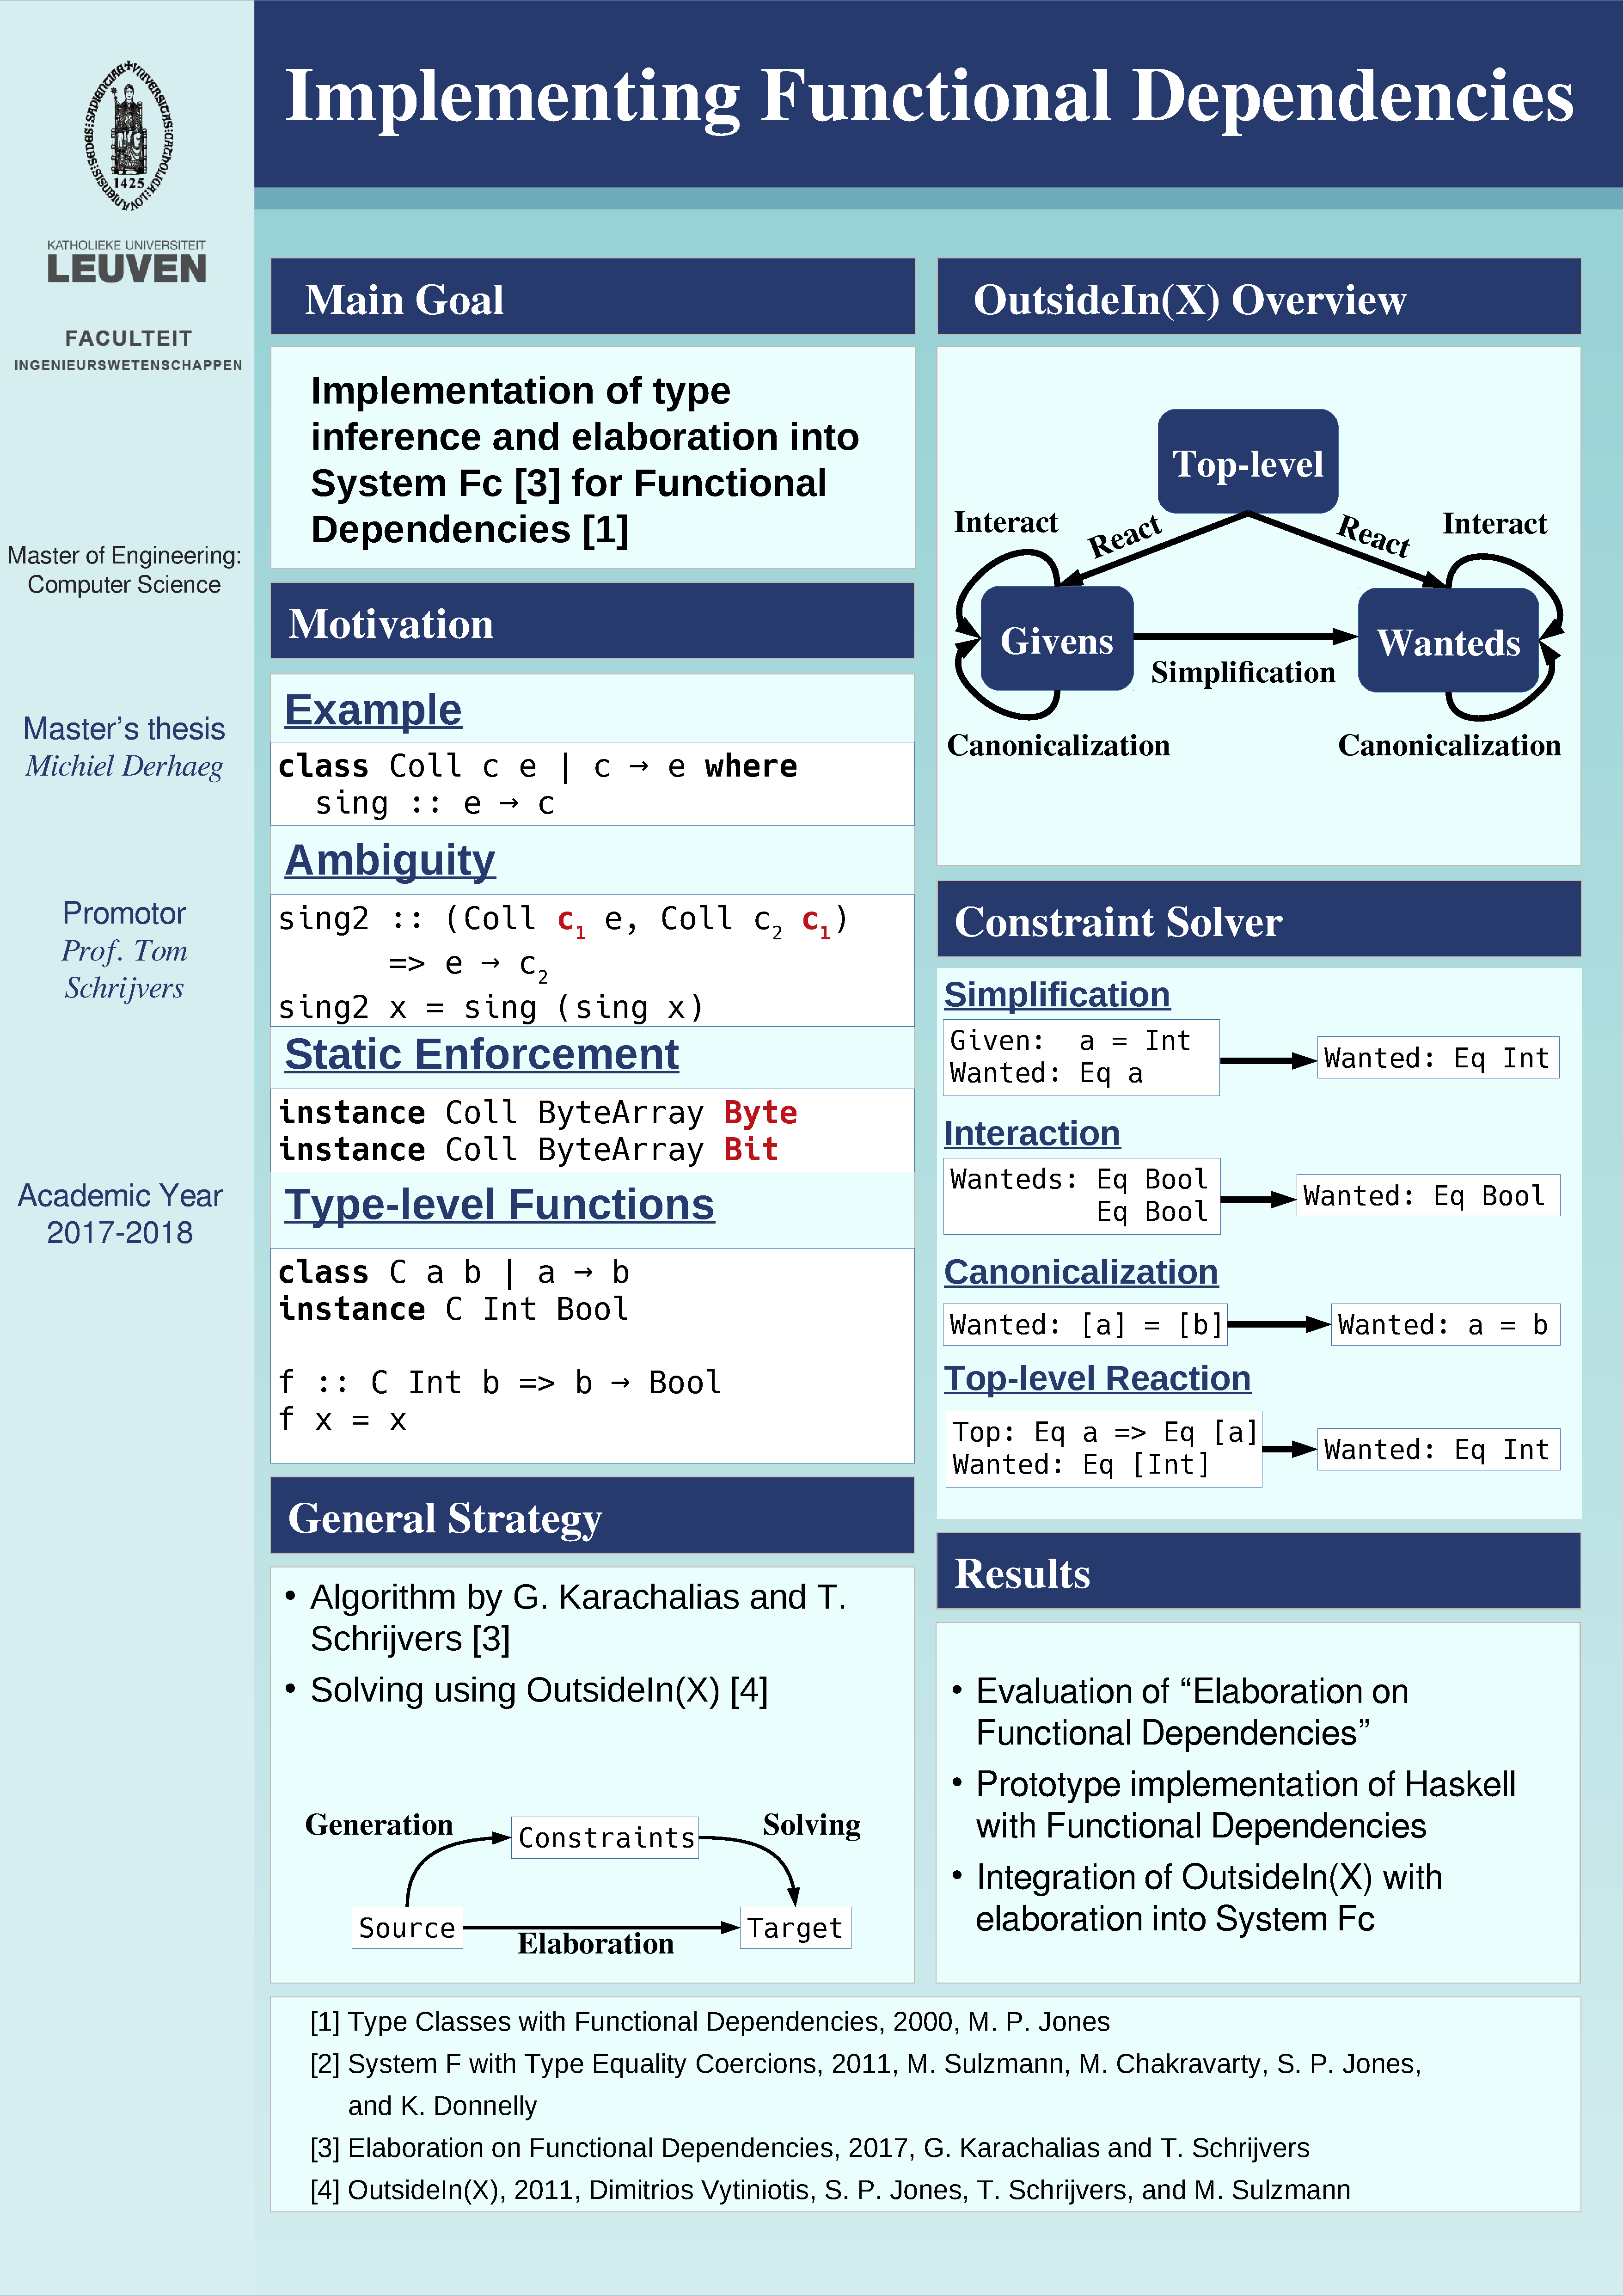
\includepdf[pages=-]{poster.pdf}
